\section{Charged Particle Tracking}

The CLAS12~\cite{Burkert:2020akg} forward detector is built around a six-coil toroidal magnet which divides the active detection area into six azimuthal regions, called ``sectors''. Each sector is equipped with three regions of drift chambers~\cite{Mestayer:2020saf} designed to detect charged particles produced by the interaction of an electron beam with a target. Each region consists of two chambers (called super-layers), each of them having 6 layers of wires. Each layer  in a super-layer contains 112 signal wires, making a super-layer a 6x112 cell matrix. The schematic view of one region  is shown on Figure~\ref{dc:side_view} (right panel).

\begin{figure}[!ht]
\begin{center}
 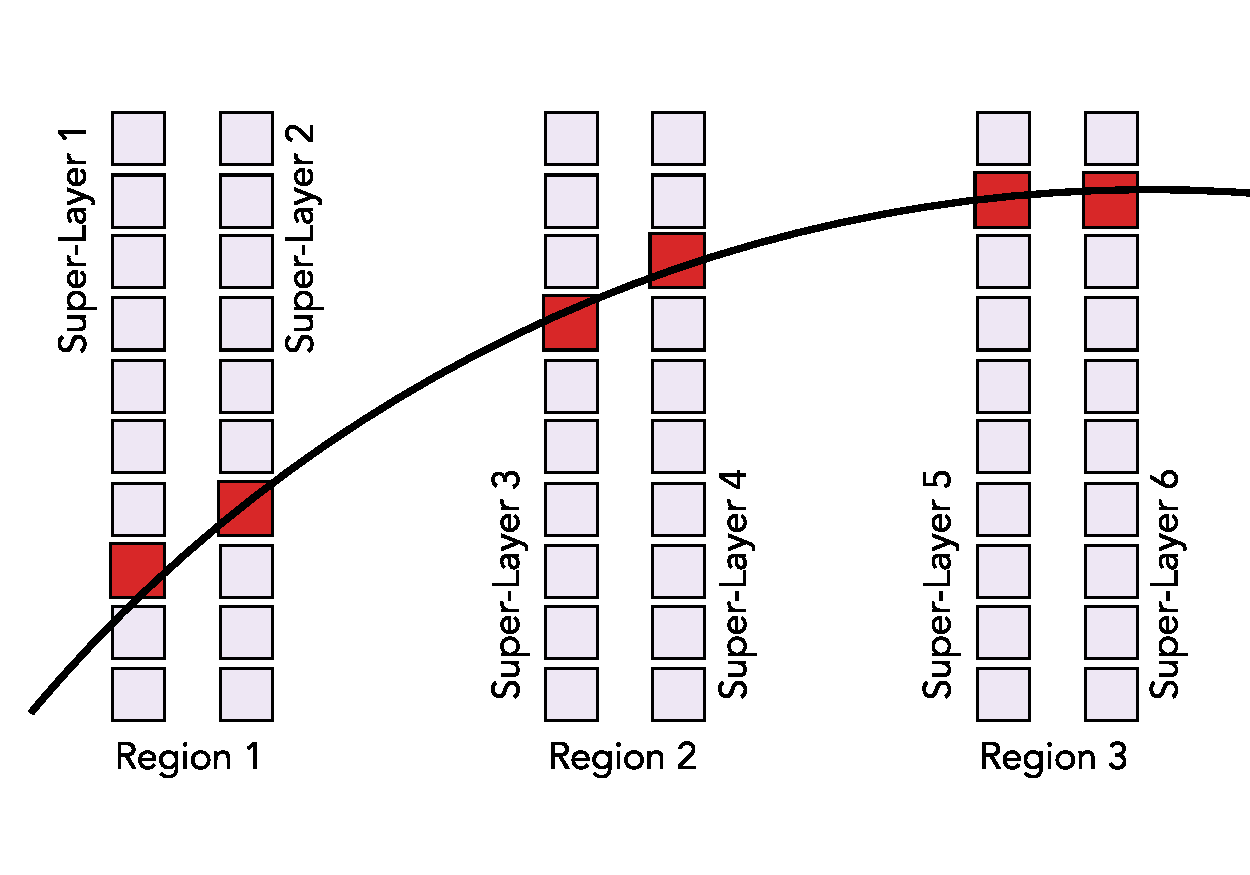
\includegraphics[width=3.1in]{images/dc_diagram.pdf}
% 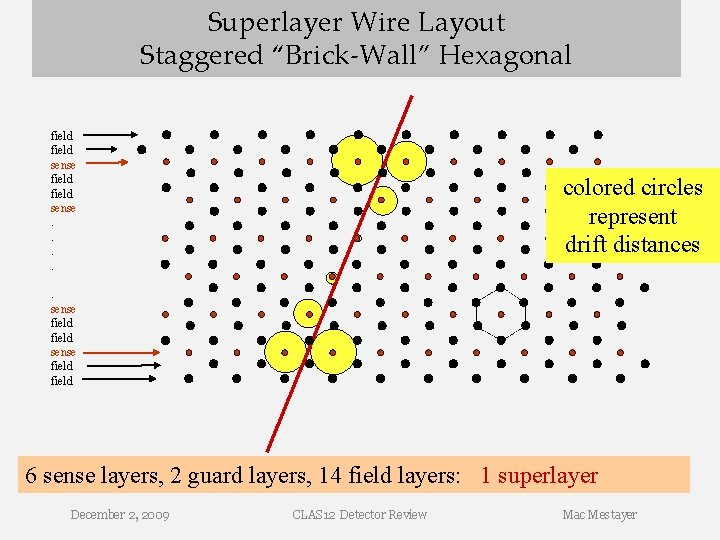
\includegraphics[width=2.5in]{images/image-29.jpg}
 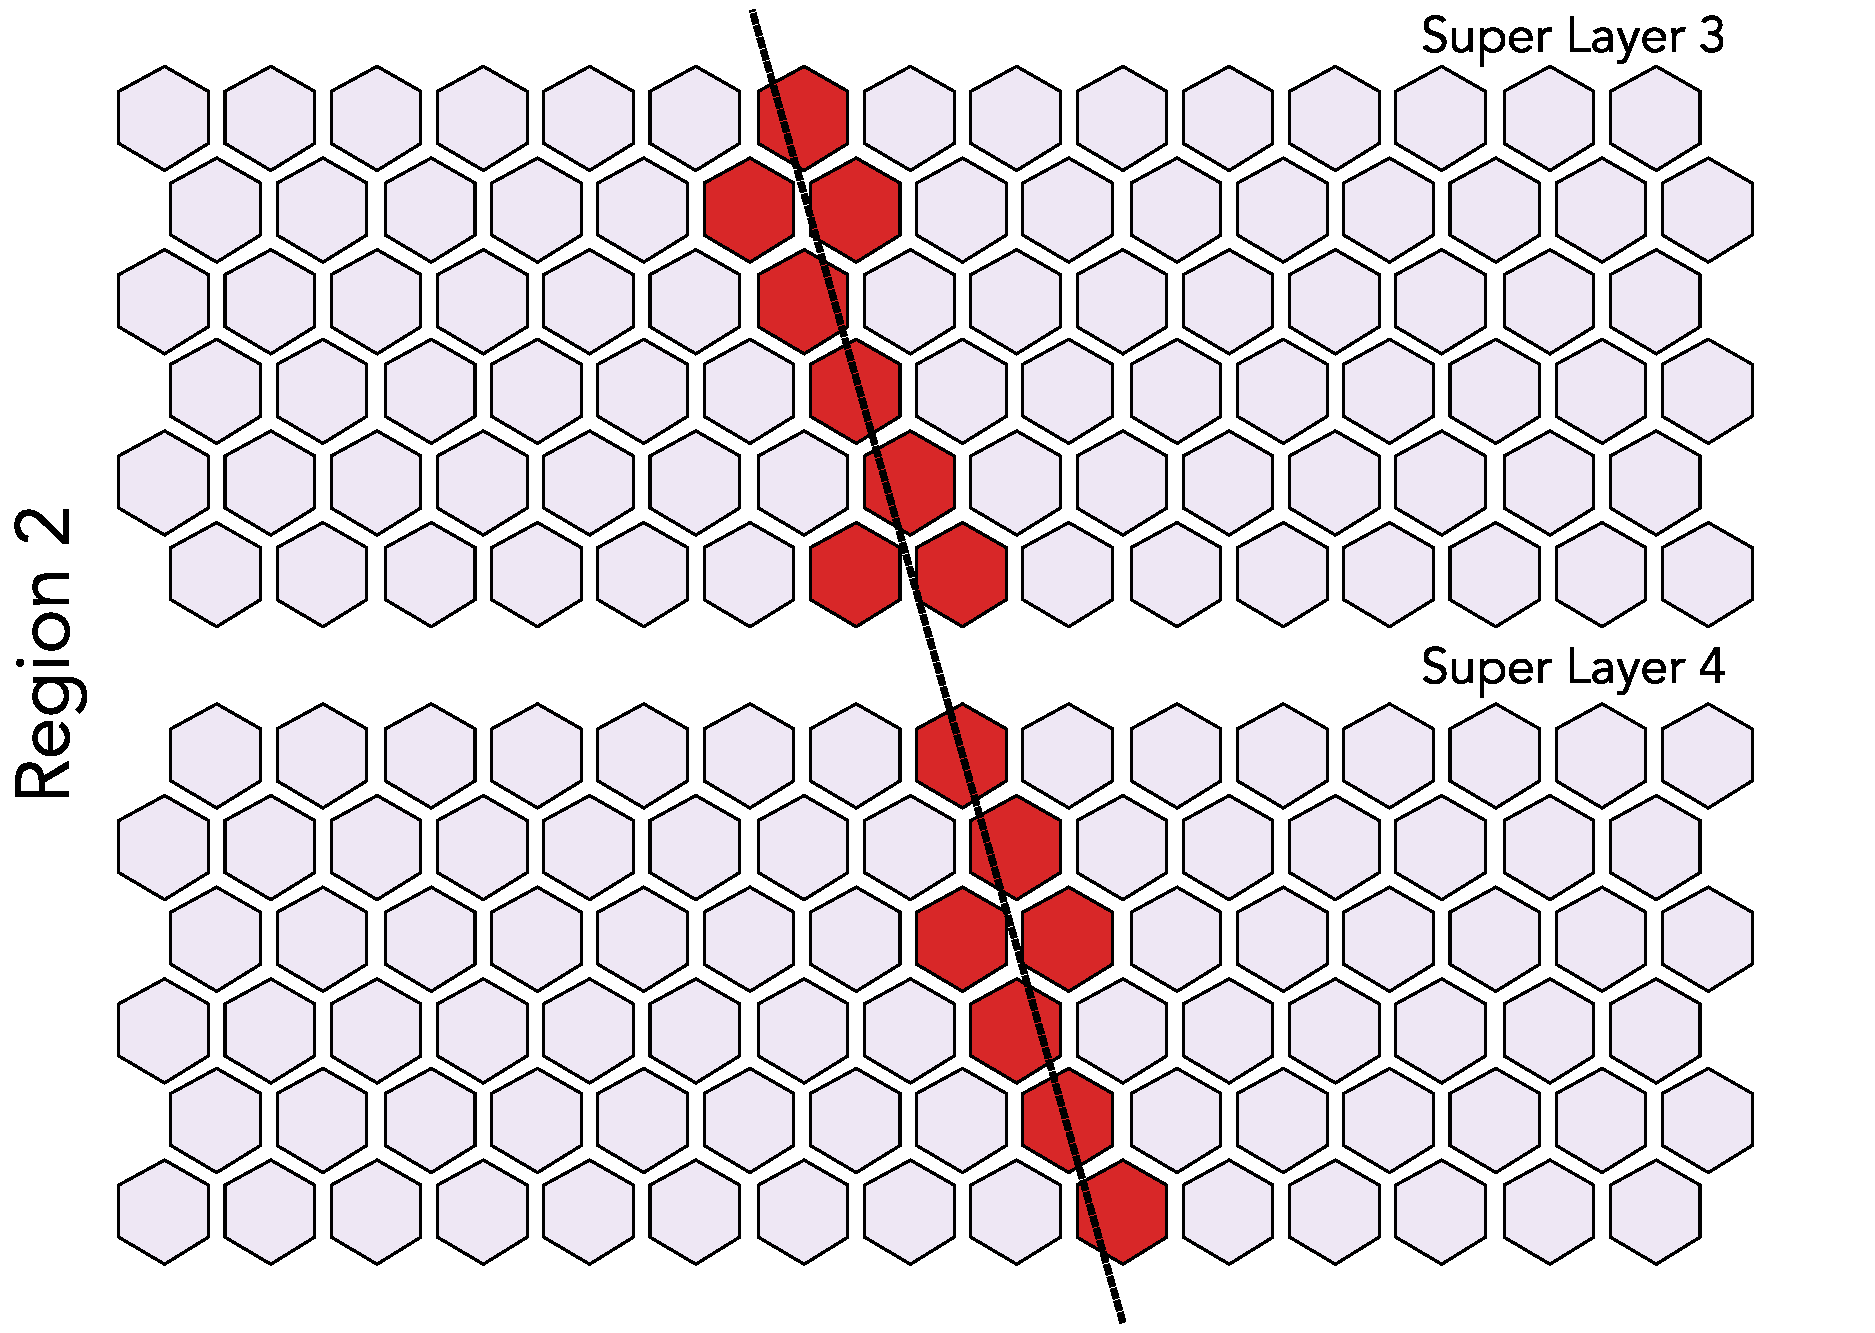
\includegraphics[width=3in]{images/region_2_diagram.pdf}
\caption {Schematic view of signals generated in the drift chambers when a particle passes through. The segments in each super-layer are shown along the trajectory of the track (left panel), and view of the activated cells in the two super-layers of one region along the track trajectory (right panel).}
 \label{dc:side_view}
 \end{center}
\end{figure}

Particles that originate at the interaction vertex travel through magnetic field and pass through all three regions of the drift chamber in a given sector are reconstructed by tracking algorithms. First, in each super-layer adjacent  with a signal are grouped together into clusters (called segments), shown on Figure~\ref{dc:side_view}. 
%Tracks passing through all regions of drift chambers leave a signal in all six super-layers schematically shown on Figure~\ref{dc:side_view} (left panel). 
 The positions of these segments (clusters) in each super-layer are used to fit the track trajectory to derive initial parameters, such as momentum and direction. After the initial selection, good track candidates are passed through Kalman filter to further refine measured parameters.

\begin{figure}[!ht]
\begin{center}
 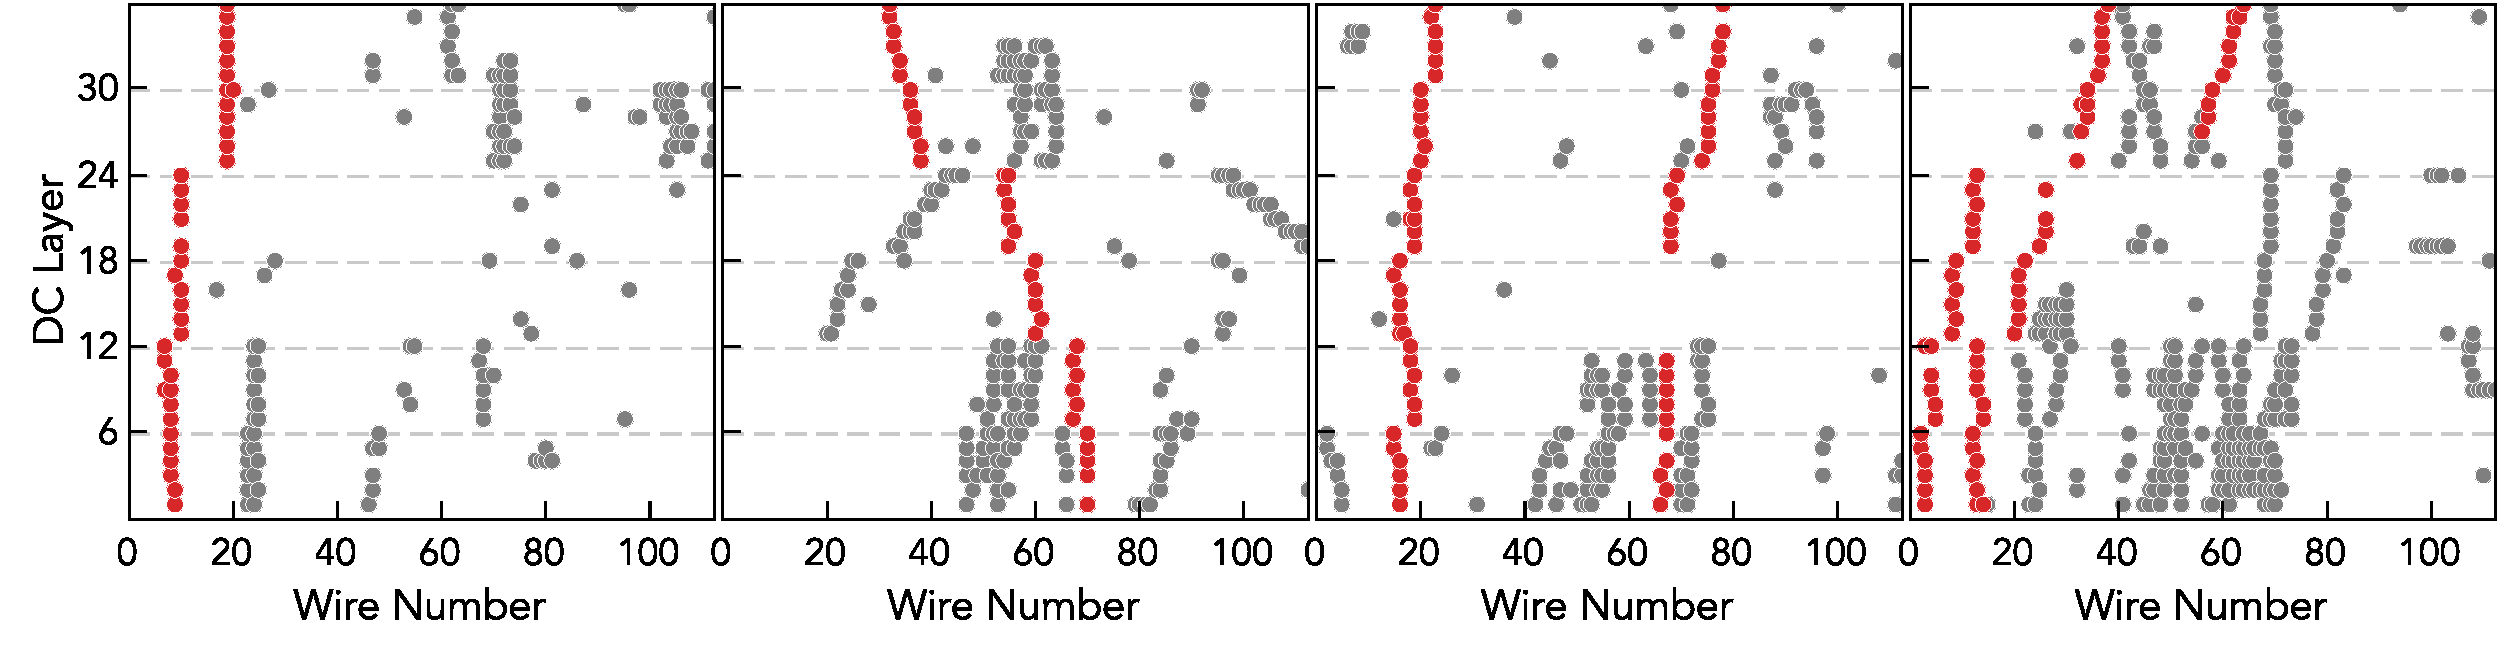
\includegraphics[width=6.2in]{images/figure_dc_examples.pdf}
\caption {Example of signals in drift chambers for few events. Each plot represents one sector with a 36x112 matrix of wires. Background hits (in gray) are shown along with the hits of reconstructed identified tracks (in red). Dashed lines represent boundaries between super-layers.}
 \label{dc:events_sector}
 \end{center}
\end{figure}

For each beam-target interaction or ``event'', drift chambers produce many segments, some belonging to a track and some to background, or partial trajectories of low momentum tracks. In Figure~\ref{dc:events_sector} drift chamber signals in one sector are shown for four different  events, in each sector data are hits represented as a 36x112 matrix (36 layers and 112 wires per layer), showing all hits including those that were determined to be part of a track. 

%At the beginning of the tracking process hits in each super-layer are analyzed to group them into clusters (segments), similar to those shown on Figure~\ref{dc:side_view} (right panel). Then, each combination of 6 segments is considered as a track candidate, and fitted to extract track parameters and goodness of fit. Candidates that pass some criteria are saved for further processing with Kalman filter. 

Due to inefficiencies in the drift chambers, it is possible to have one missing segment along the trajectory of the particle, and the track has to be reconstructed using only 5 segments. An example of a 5-segment track is shown on Figure~\ref{dc:events_sector} c), where super-layer 3 does not have any segment detected. For these types of tracks, candidates have to be identified from a large number of combinatorics consisting of all combinations of clusters that form a  5-segment candidates. 

Tracking is computationally extensive and makes up $80\%-90\%$ (depending on background conditions and track multiplicity) of the total CLAS12 event processing time. The procedure of finding tracks from a list of track candidates is where we found AI can provide real benefits. Such benefits include: improved accuracy in identifying good tracks, and improved data processing speed by significantly reducing the number of candidates that have to go through initial fitting and then through Kalman filter. AI can also help in identifying 5 super-layer track candidates.

 %When reconstructing tracks in the event many combinations of segments have to be considered to determine which one represents a valid track trajectory. 
%then track candidates are constructed by forming 6 segment combinations (one per each super-layer). Each track candidate is validated by tracking algorithm by performing a polynomial fit to determine if the candidate can be a real track. Once track candidates are isolated they are further refined using Kalman filter to measure particle parameters (such as momentum and angles). 
%There are many experiments conducted with CLAS12 detector which have different running conditions (i.e. different targets and beam currents).
%The changing beam energies and beam intensities (current) affect the amount of background that is detected in each detector components. For drift chambers the added background can be in a form of random hits that can be isolated by noise reducing algorithm, and can be in form of segments that do not belong to a track. With increased luminosity (beam current and target combination) number of combinatorics and the candidates to consider significantly increases, and this leads to decreased efficiency in track reconstruction. Recent studies done with experimental data and simulation showed that the tracking efficiency decreases with a rate of $0.44\%$ per nA of beam current. This leads to tracking efficiency at standard experimental running conditions (which is $45~nA$ electron beam incident on $40~cm$ liquid hydrogen target) is $\approx 80\%$.
%The decrease of the efficiency of tracking what prevents experiments to run at higher beam currents (interaction rates), and increasing tracking efficiency will allow experiments to run for shorter time to collect desired statistics for physics results. 